\section{\textbf{Capitolo 2}}
\underline{Le funzioni usate nei codici seguenti sono in fondo al capitolo}
\subsection{Esercizio 1}
Per ricercare la radice quadrata di un numero è possibile sfruttare una modifica al problema delle radici di una funzione. Infatti partendo da $x=\sqrt{\alpha}$ è possibile svilupparla trovando una funzione $f(x)$ utilizzabile nel metodo di Newton:
\[
x = \sqrt{\alpha} 
\]
\[
x^{2} = \big(\sqrt{\alpha}\big)^{2} 
\]
\[
x^{2} - \alpha = 0
\]
possiamo quindi considerare $f(x) = x^{2} - \alpha$ e $f'(x) = 2\cdot x$ . La procedura iterativa è definita quindi da:
\[
x_{n+1} = x_{n} - \frac{f(x_{n})}{f'(x_{n})} = x_{n}-\frac{x_{n}^2-\alpha}{2\cdot x_{n}} = x_{n} - \frac{x_{n}}{2} + \frac{\alpha}{2\cdot x_{n}} = \frac{x_{n}}{2}+\frac{\alpha}{2\cdot x_{n}} = \frac{1}{2} \cdot \Big(x_{n}+\frac{\alpha}{x_{n}}\Big)
\]
che ci permette di implementare il seguente script matlab e la funzione y = NewtonSqrt(alpha, x\_0, imax, tol):
\lstinputlisting[language=matlab]{cap_2/es1/es1.m}
Che restituisce in output valori che abbiamo rappresentato nella tabella seguente:
\begin{center}
\begin{tabular}{|c|c|}
\hline
$i$ & \( x_i \) \\
\hline
1 & 1.750000000000000e+00 \\
2 & 1.732142857142857e+00 \\
3 & 1.732050810014727e+00 \\
4 & 1.732050807568877e+00 \\
\hline
\end{tabular}\\
\end{center}
\subsection{Esercizio 2}
\begin{flushleft}
E' possibile effettuare gli stessi passaggi dell'esercizio precedente, ricordandosi che la radice in questo caso non è quadrata ma ennesima:
\[
x = \sqrt[n]{\alpha} 
\]
\[
x^{n} = \big(\sqrt[n]{\alpha}\big)^{n} 
\]
\[
x^{n} - \alpha = 0
\]
consideriamo quindi la funzione $f(x) = x^{n} - \alpha$ e $f'(x) = n\cdot x^{n-1}$ . La procedura iterativa è definita quindi da:
\[
x_{n+1} = x_{n} - \frac{f(x_{n})}{f'(x_{n})} = x_{n}-\frac{x_{n}^n-\alpha}{n\cdot x_{n}^{n-1}} = x_{n} - \frac{x_{n}}{n} + \frac{\alpha}{n\cdot x_{n}^{n-1}} = 
\]
\[
= \Big((n-1)\cdot x_n- \frac{\alpha}{x_n^{n-1}}\Big) \cdot \frac{1}{n} = \frac{\Big( (n-1)\cdot x_n^{n}+\alpha\Big)}{n\cdot x_n^{n-1}}
\]
La radice da approssimare in questo caso ha grado ennesimo quindi sono necessarie delle modifiche alla funzione matlab usata nell'esercizio precedente che chiamiamo y = NewtonSqrt(n, alpha, x\_0, imax, tol). Lo script MatLab corrispondente ai casi $n = 3,4,5$ è il seguente:
\lstinputlisting[language=Matlab]{cap_2/es2/es2.m}
Mostriamo l'output in forma tabellare con $i$ che rappresenta le iterazioni del metodo e $x_i$ i relativi risultati:
\begin{center}
\begin{tabular}{|c|c|c|c|}
\hline
i & $x_i$ con $n=3$ & $x_i$ con $n=4$ & $x_i$ con $n=5$\\
\hline
1 & 1.631784138709347e+00 & 1.771797299323380e+00 & 1.943788863498140e+00 \\
2 & 1.463411989089094e+00 & 1.463688102853308e+00 & 1.597060655491283e+00 \\
3 & 1.442554125137959e+00 & 1.336940995805593e+00 & 1.369877122538772e+00 \\
4 & 1.442249634601091e+00 & 1.316557487370408e+00 & 1.266284124539191e+00 \\
5 & 1.442249570307411e+00 & 1.316074279204018e+00 & 1.246387399421677e+00 \\
6 & ------------ & 1.316074012952573e+00 & 1.245731630753065e+00 \\
7 & ------------ & ------------ & 1.245730939616284e+00 \\
\hline
\end{tabular}
\end{center}
\end{flushleft}
\subsection{Esercizio 3}
Per confrontare il metodo delle secanti con quello di Newton abbiamo creato il codice MatLab:
\lstinputlisting[language=matlab]{cap_2/es3/es3.m}
I risultati ottenuti dall'utilizzo del metodo delle secanti sono: \newline
\\
\scalebox{0.9} {
\begin{tabular}{c|c|c|c|c}
i & metodo di Newton & metodo delle secanti & \big|newton-$\sqrt{2}$\big| & \big|secanti-$\sqrt{2}$\big|\\
\hline
1 & 1.750000000000000e+00 & 1.736842105263158e+00 & 3.357864376269049e-01 & 3.226285428900628e-01 \\
2 & 1.732142857142857e+00 & 1.732142857142857e+00 & 3.179292947697618e-01 & 3.179292947697618e-01 \\
3 & 1.732050810014727e+00 & 1.732050934706042e+00 & 3.178372476416318e-01 & 3.178373723329468e-01 \\
4 & --------- & 1.732050807572255e+00 & ------- & 3.178372451991598e-01\\
\end{tabular}
}
\\ \newline
Si nota dalla tabella che \( \big|newton-\sqrt{2}\big| \approx  \big|secanti-\sqrt{2}\big| \), cioè che l'ordine di grandezza dell'errore assoluto tra i due metodi è lo stesso. Si può quindi affermare che l'uso del metodo di Newton o del metodo delle secanti è equivalente.
\newpage
\subsection{Esercizio 4}
\begin{flushleft}
Abbiamo scritto delle funzioni MalLab che ci permettono di effettuare il raffronto tra i vari metodi (in ordine: metodo di Newton, metodo di Newton modificato, metodo di accelerazione di Aitken), è possibile vederle a pag. \pageref{functcap2}. Scritte le Function, le abbiamo usate nel seguente script: 
\lstinputlisting[language=Matlab]{cap_2/es4/es4.m}
Questo codice esegue i metodi di Newton, Newton modificato e Aitken per le funzioni date. Rispetto alla funzione $f_1(x)=(x-\pi)^{10}$ rappresentiamo l'output del codice precedente in forma tabellare: 
\begin{center}
\begin{tabular}{|c|c|c|c|}
\hline
tolx & Newton & Newton modificato & Aitken \\
\hline
$10^{0}$ & 4.814159265358979 & 4.814159265358979 & 2.666666666666667 \\
$10^{-1}$ & 4.030463126315021 & 4.030463126315021 & 3.141592653589783 \\
$10^{-2}$ & 3.229126031324792 & 3.229126031324792 & 3.141592653589783 \\
$10^{-3}$ & 3.150212685926121 &  3.150212685926121 &  3.141592653589783 \\ 
$10^{-4}$ & 3.150212685926121 & 3.150212685926121 & 3.141592653589783 \\
$10^{-5}$ & 3.150212685926121 & 3.150212685926121 & 3.141592653589783 \\
\hline
\end{tabular}
\end{center}
Rispetto alla funzione $f_2(x) = (x-\pi)^{10} \cdot e^{2\cdot x}$ si hanno invece i valori:
\begin{center}
\begin{tabular}{|c|c|c|c|}
\hline
tolx & Newton & Newton modificato & Aitken \\
\hline
$10^{0}$ & 4.864516114854061 & 4.864516114854061 & 3.068982105941251 \\
$10^{-1}$ & 4.200823975656096 & 4.200823975656096 & 3.140645194956157 \\
$10^{-2}$ & 3.226469748549500 & 3.226469748549500 & 3.141592492095279 \\
$10^{-3}$ & 3.154537411727535 & 3.154537411727535 &  3.141592492095279 \\ 
$10^{-4}$ & 3.154537411727535 & 3.154537411727535 & 3.141592516390607 \\
$10^{-5}$ & 3.154537411727535 & 3.154537411727535 & 3.141592516390607 \\
\hline
\end{tabular}
\end{center}
Abbiamo poi riportato il plot matlab relativo ai precedenti valori:
\begin{figure}[H]
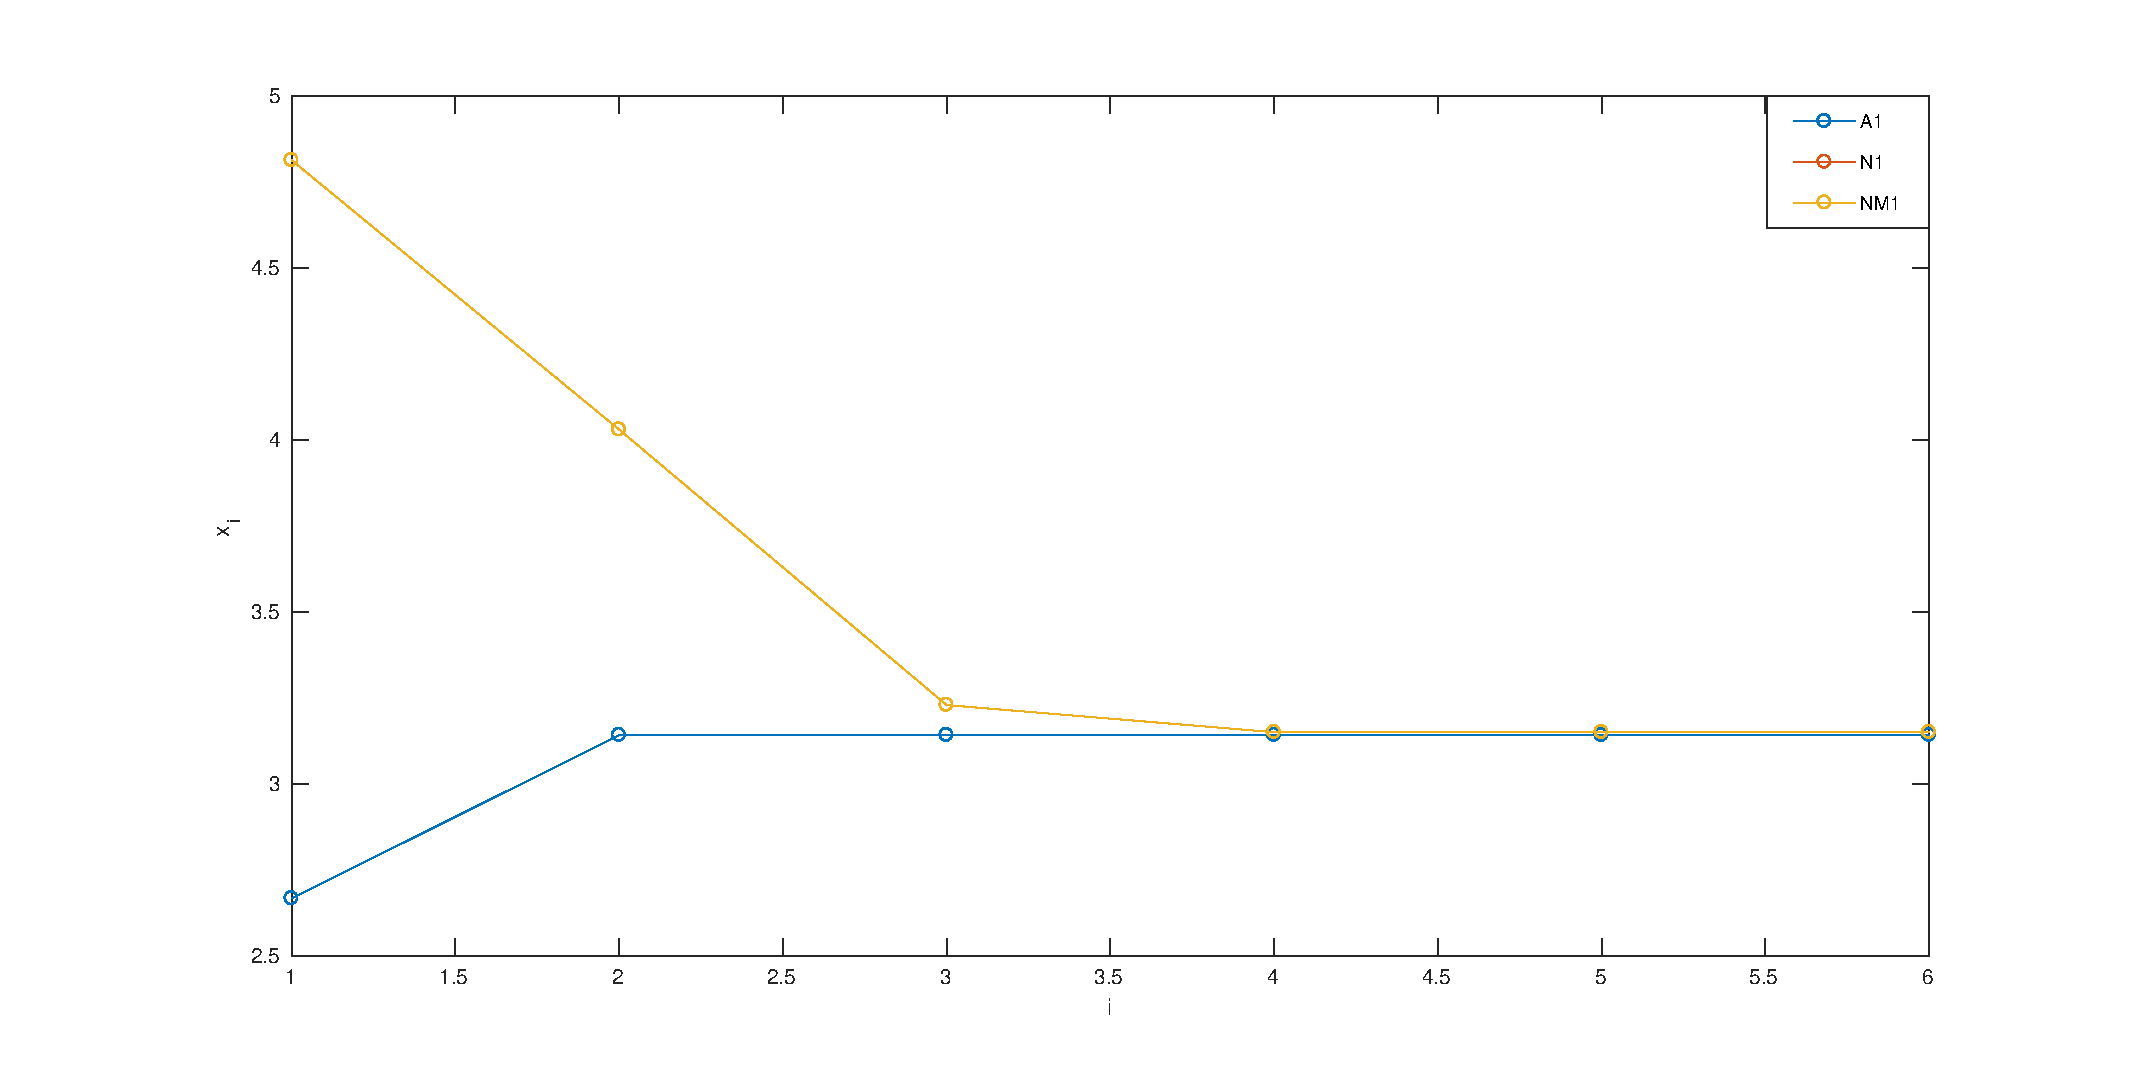
\includegraphics[left, width=210px]{plot/fes24a.eps}
\caption{Andamento del calcolo degli zeri della funzione $f_1(x)=(x-\pi)^{10}$ al variare della tolleranza}
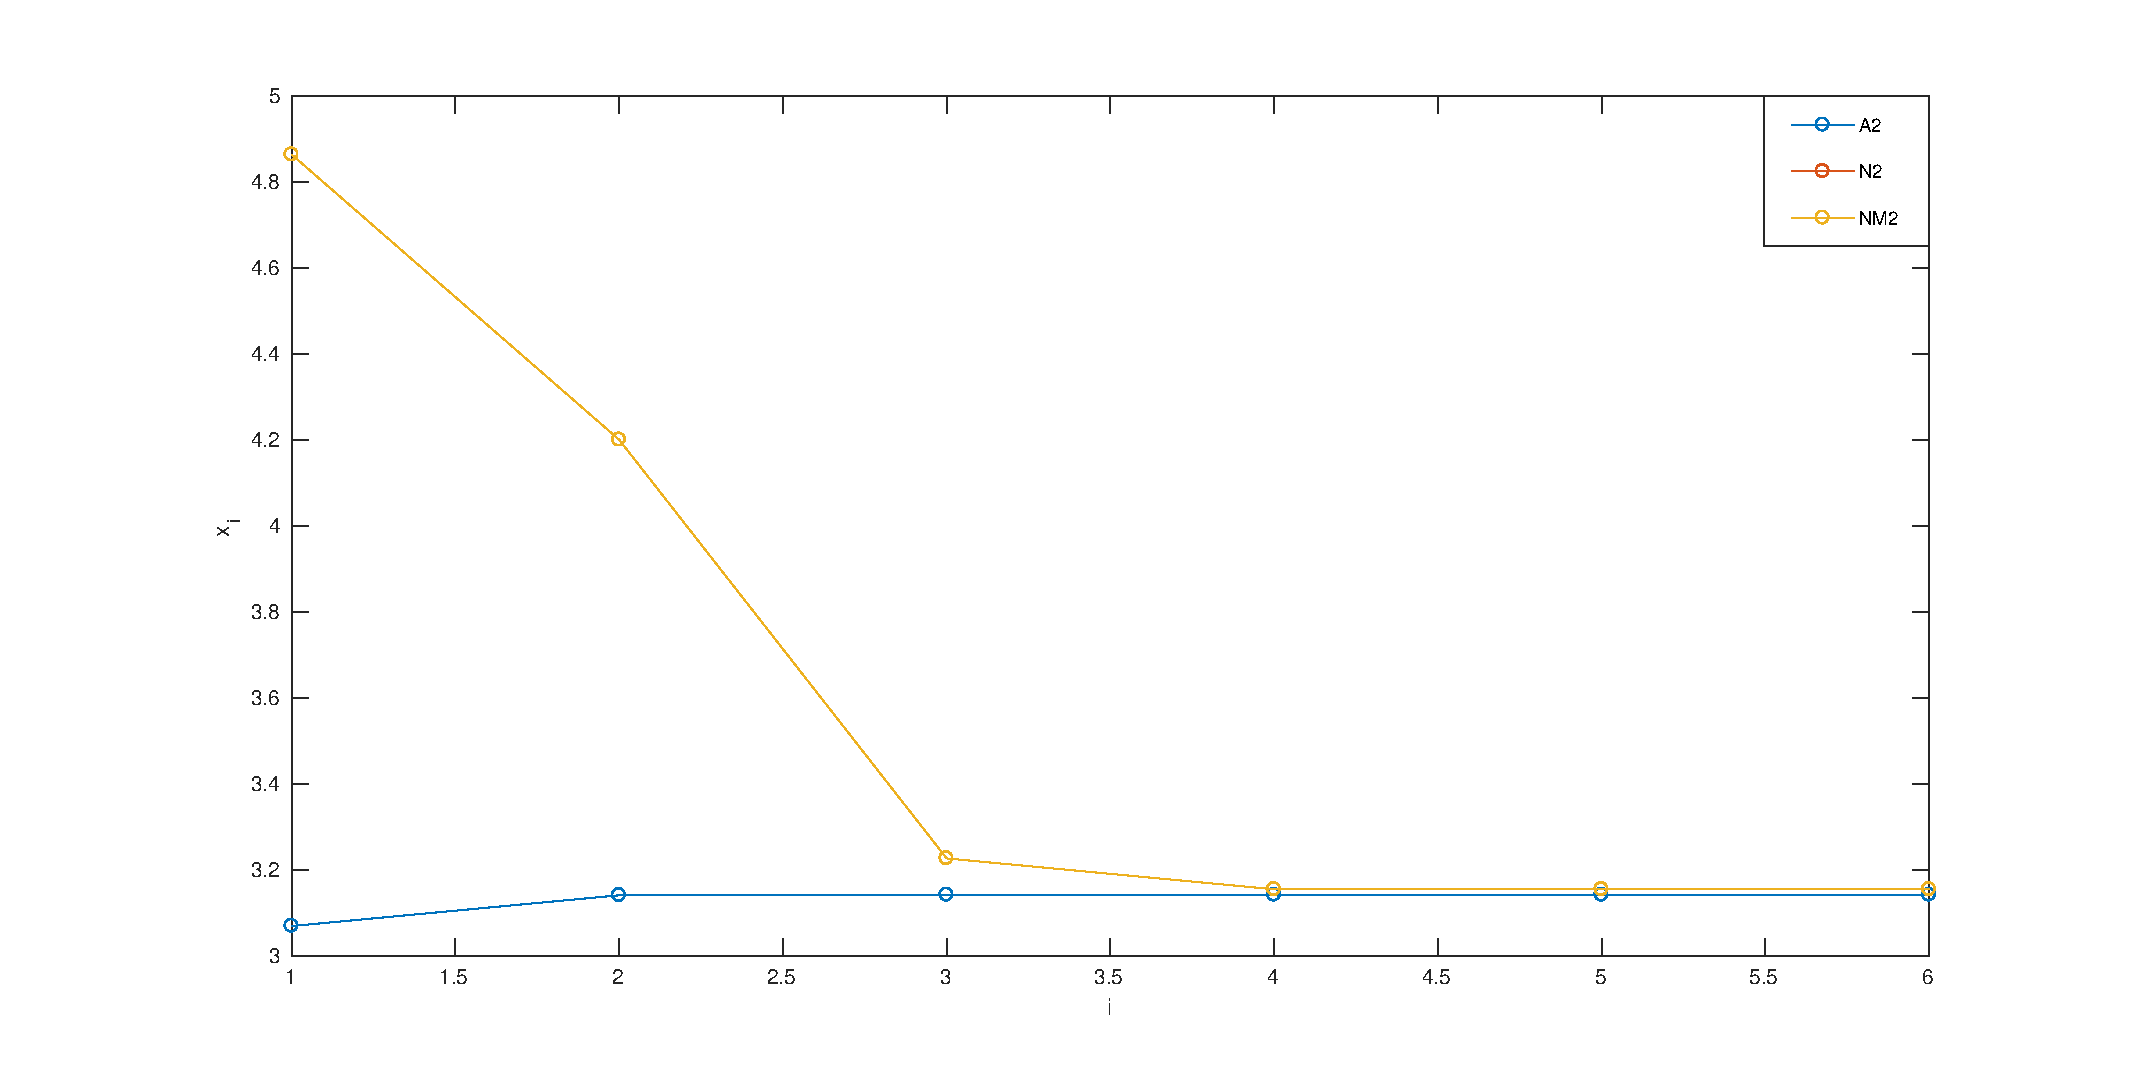
\includegraphics[left, width=210px]{plot/fes24b.eps}
\caption{Andamento del calcolo degli zeri della funzione $f_2(x) = (x-\pi)^{10} \cdot e^{2\cdot x}$ al variare della tolleranza}
\end{figure}
\end{flushleft}
\subsection{Esercizio 5}
Il metodo di bisezione \'e applicabile se la funzione \(f\) \'e
\begin{enumerate}

\item continua nell'intervallo \( [a,b] \)
\item tale che \( f(a)f(b)<0 \)

\end{enumerate}

Dal momento che lo zero delle funzioni \( f_1(x)=(x-\pi)^{10} \) e \( f_2(x)=e^{2x}(x-\pi)^{10} \) risulta essere in \( x=\pi \), ultilizzare come punto iniziale \( x_0 = 5 > \pi \) non porterebbe chiaramente alla determinazione dello zero ancor prima di valutare la regolarit\'a della funzione. 
Analizzando poi le due \( f \) si nota subito che \[
\nexists x | f_1(x)<0, \forall x \in \mathbb{R}, \]
\[
\nexists x | f_2(x)<0, \forall x \in \mathbb{R}.
\]


\begin {flushleft} Dal momento che queste sono funzioni esponeziali con minimo \(x_{min} = \pi \), risulta evidente come il suddetto metodo non sia applicabile. \end{flushleft}
 


\subsection{Esercizio 6}
\begin{flushleft}
Per poter costruire una tabella abbiamo scritto il seguente codice MatLab (lo script usa function definite a parte che è possibile vedere a pagina \pageref{functcap2}):
\lstinputlisting[language=Matlab]{cap_2/es6/es6.m}
Sotto forma tabellare rappresentiamo il numero di iterazioni effettuate dai 3 algoritmi (salvate nella matrice $iter$):

\begin{center}
\begin{tabular}{|c|c|c|c|}
\hline
$tol_x$ & Newton & Secanti & Corde \\
\hline
$10^{-1}$ & 2 & 3 & 2 \\
$10^{-2}$ & 3 & 3 & 8 \\
$10^{-3}$ & 3 & 4 & 15 \\
$10^{-4}$ & 3 & 5 & 22 \\
$10^{-5}$ & 4 & 5 & 28 \\
$10^{-6}$ & 4 & 5 & 35 \\
$10^{-7}$ & 4 & 5 & 42 \\
$10^{-8}$ & 4 & 6 & 48 \\
$10^{-9}$ & 4 & 6 & 55 \\
$10^{-10}$ & 5 & 6 & 62 \\
\hline
\end{tabular}
\end{center}
Questo risultato è possibile vederlo tramite il plot MatLab:
\begin{figure}[H]
\label{fes26}
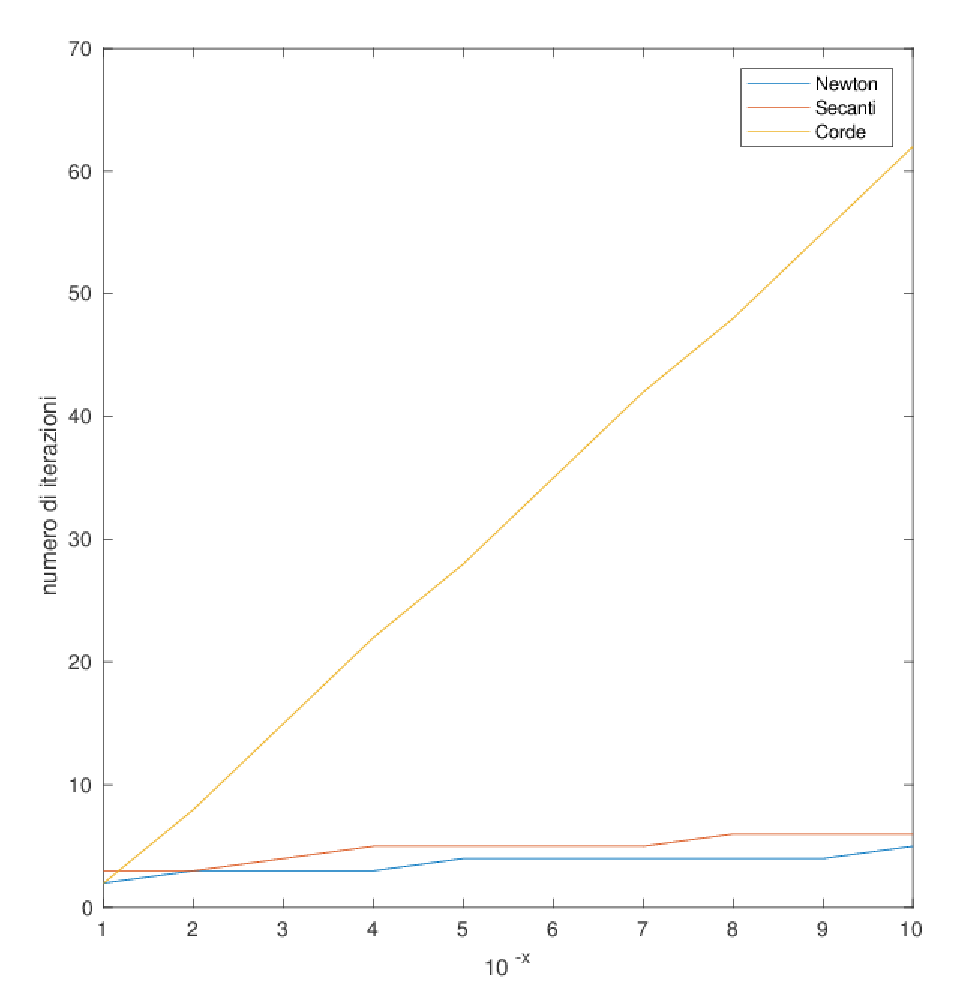
\includegraphics[width=480px, height=280px]{plot/fes26}
\caption{\texttt{\texttt{Andamento del numero delle iterazioni al decrescere della tolleranza per i metodi Newton, Secanti, Corde}}}
\end{figure}
Il numero di condizionamento del problema è dato da:
\[
k = \frac{1}{\big|f'(x^*)\big|}
\]
Per poterlo calcolare è necessario trovare la derivata della nostra funzione che è pari a:
\[
f'(x) = -1 - cos(x) + 5 \cdot sin(10\cdot x) - \frac{cos^2(10\cdot x)}{2}
\]
Essendo la radice della nostra funzione  $x^* = 0,488944$ il relativo numero di condizionamento è dato da:
\[
k = \frac{1}{\Big|f'(x^*)\Big|} = \frac{1}{\Big|f'(0,488944)\Big|} = \frac{1}{\Big|-4,27233\Big|} = \frac{1}{4,27233} = 0,234064
\]
questo significa che il problema è ben condizionato.
\end{flushleft}
\newpage
\subsection{Esercizio 7}
\begin{flushleft}
Lo script usato è il seguente:
\lstinputlisting[language=MatLab]{cap_2/es7/es7.m}
\lstinputlisting[language=matlab]{cap_2/bisect.m}
Il numero di iterazioni del metodo di bisezione risultanti sono:

\begin{center}
\begin{tabular}{|c|c|c|c|}
\hline
$tol_x$ & bisezione \\
\hline
$10^{-1}$ & 2 \\
$10^{-2}$ & 7 \\
$10^{-3}$ & 10 \\
$10^{-4}$ & 14 \\
$10^{-5}$ & 17 \\
$10^{-6}$ & 20 \\
$10^{-7}$ & 24 \\
$10^{-8}$ & 27 \\
$10^{-9}$ & 30 \\
$10^{-10}$ & 34 \\
\hline
\end{tabular}
\end{center}

Si può vedere dal grafico l'andamento dei vari metodi usati nel seguente plot MatLab:
\begin{figure}[H]
\label{fes27}
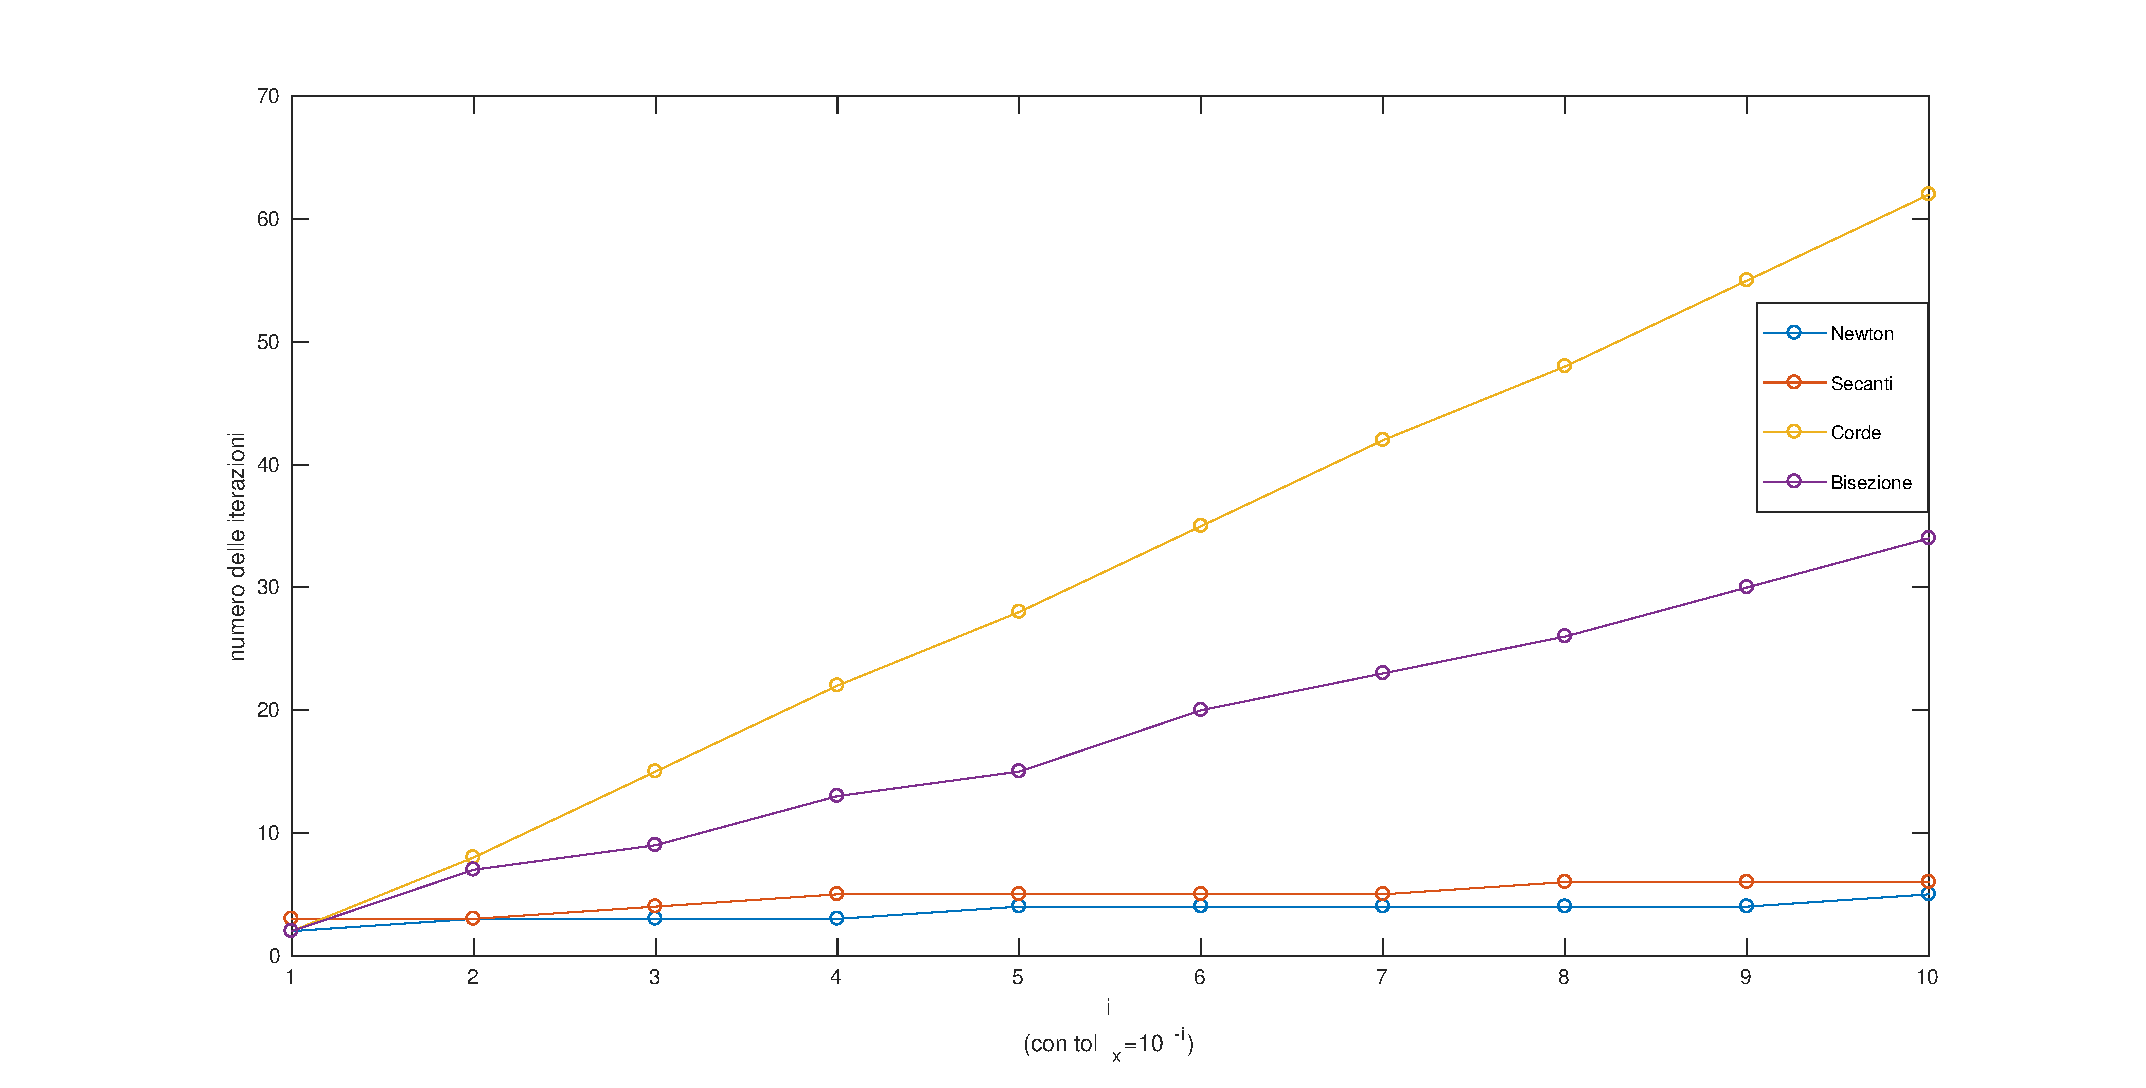
\includegraphics[width=480px, height=280px]{plot/fes27}
\caption{\texttt{Aggiunta dell'andamento del metodo di Bisezione rispetto ai precedenti metodi}}
\end{figure}

\end{flushleft}
\newpage
\subsection{Esercizio 8}
\lstinputlisting[language=Matlab]{cap_2/es8/es8.m}

Essendo \[f'(x)=10(x-\pi)^{10x}(\frac{x}{x-\pi}+\ln{(x-\pi)})\]
E dato che quest'ultima contiene $ln(x - \pi)$, il cui dominio \'e \( \{ \forall x \in \mathbb{R} | x > \pi \}\), il metodo non potrà convergere per valori di $x_0 \leq \pi$

\subsection{Funzioni MatLab Usate}
\label{functcap2}
\subsubsection{Metodo Newton per $\sqrt{\alpha}$}
\lstinputlisting[language=matlab]{cap_2/NewtonSqrt.m}
\subsubsection{Metodo Newton per $\sqrt[n]{\alpha}$}
\lstinputlisting[language=matlab]{cap_2/NewtonSqrtN.m}
\subsubsection{Metodo delle secanti per $\sqrt{\alpha}$}
\lstinputlisting[language=matlab]{cap_2/SecSqrt.m}
\subsubsection{Metodo di Newton}
\lstinputlisting[language=matlab]{cap_2/Newton.m}
\subsubsection{Metodo di Newton Modificato}
\lstinputlisting[language=matlab]{cap_2/NewtonMod.m}
\subsubsection{Metodo di accelerazione di Aitken}
\lstinputlisting[language=matlab]{cap_2/Aitken.m}
\subsubsection{Metodo delle secanti}
\lstinputlisting[language=matlab]{cap_2/secanti.m}
\subsubsection{Metodo delle corde}
\lstinputlisting[language=matlab]{cap_2/corde.m}
\subsubsection{Metodo della bisezione}
\lstinputlisting[language=matlab]{cap_2/bisect.m}